\documentclass[10pt]{beamer}

\usepackage{iftex,ifxetex}
\ifPDFTeX
  \usepackage[utf8]{inputenc}
  \usepackage[T1]{fontenc}
  \usepackage[russian]{babel}
  \usepackage{lmodern}
  \usefonttheme{serif}
\else
  \ifluatex
    \usepackage{unicode-math}
    \defaultfontfeatures{Ligatures=TeX,Numbers=OldStyle}
    \setmathfont{Latin Modern Math}
    \setsansfont{Linux Biolinum O}
    \setmonofont{Fira Code}
    \usefonttheme{professionalfonts}
    % \setmathfont[
    %     Ligatures=TeX,
    %     Scale=MatchLowercase,
    %     math-style=upright,
    %     vargreek-shape=unicode
    %     ]{euler.otf}
  \fi
\fi


\usepackage{amsmath,amssymb,longtable,hhline}
\usepackage{mathrsfs}
\usepackage{xcolor}
\usepackage{listings}
\usepackage{hyperref}
\usepackage{multicol}
\usepackage{anyfontsize}
\usepackage{minted}
\usepackage{tikz}
\usepackage{indentfirst}
%\usepackage{enumitem}

\usetikzlibrary{matrix}
% \setlist[description]{leftmargin=0pt,labelindent=\parindent}

\usemintedstyle{tango}
\newcommand{\ltprgsize}{\fontsize{5}{5}\selectfont}
\setminted{fontsize=\ltprgsize,mathescape}

\definecolor{mygreen}{rgb}{0,0.6,0}
\definecolor{mygray}{rgb}{0.5,0.5,0.5}
\definecolor{mymauve}{rgb}{0.58,0,0.82}

\hypersetup{
    bookmarks=true,         % show bookmarks bar?
    unicode=true,           % non-Latin characters in Acrobat’s bookmarks
    pdftoolbar=false,        % show Acrobat’s toolbar?
    pdfmenubar=false,        % show Acrobat’s menu?
    pdffitwindow=false,     % window fit to page when opened
    pdfstartview={FitH},    % fits the width of the page to the window
    pdftitle={Компьютерная алгебра в задачах оптимизации},    % title
    pdfauthor={Evgeny Cherkashin, Seseg Badmatsyrenova},     % author
    pdfsubject={symbolic computations},   % subject of the document
    pdfnewwindow=true,      % links in new PDF window
    colorlinks=true,       % false: boxed links; true: colored links
    linkcolor=red,          % color of internal links (change box color with linkbordercolor)
    citecolor=green,        % color of links to bibliography
    filecolor=magenta,      % color of file links
    urlcolor=blue           % color of external links
}

\usepackage{pifont}

\usetheme{Warsaw}
\usecolortheme{crane}
%\useinnertheme{rectangles}
\setbeamertemplate{itemize item}{\scriptsize\hbox{\donotcoloroutermaths\ding{113}}}
\setbeamertemplate{itemize subitem}{\tiny\raise1.5pt\hbox{\donotcoloroutermaths$\blacktriangleright$}}
\setbeamertemplate{itemize subsubitem}{\tiny\raise1.5pt\hbox{\donotcoloroutermaths$\blacktriangleright$}}
\setbeamertemplate{enumerate item}{\insertenumlabel.}
\setbeamertemplate{enumerate subitem}{\insertenumlabel.\insertsubenumlabel}
\setbeamertemplate{enumerate subsubitem}{\insertenumlabel.\insertsubenumlabel.\insertsubsubenumlabel}
\setbeamertemplate{enumerate mini template}{\insertenumlabel}

\beamertemplatenavigationsymbolsempty


%\useoutertheme{split}
%\useinnertheme{rounded}
\setbeamertemplate{background canvas}[vertical shading][bottom=white!80!cyan!20,top=cyan!10]
%\setbeamertemplate{sidebar canvas left}[horizontal shading][left=white!40!black,right=black]

\graphicspath{{pics/}}


% --------------------------

% Продукт (Конкуренты, свойства)
% Графический аспект
% Технические аспекты
% Содержание сайта
% Дополнительная информация
% Контактная информация


  \tikzset{
    table/.style={
        matrix of nodes,
        row sep=-\pgflinewidth,
        column sep=-\pgflinewidth,
        nodes={
            rectangle,
            draw=black,
            align=center
        },
        minimum height=1.5em,
        text depth=0.5ex,
        text height=2ex,
        nodes in empty cells,
%%
        every even row/.style={
            nodes={fill=gray!20}
        },
        column 1/.style={
 %           nodes={text width=2em,font=\bfseries}
            nodes={font=\bfseries}
        },
        row 1/.style={
            nodes={
                % fill=black,
                % text=white,
                font=\bfseries
            }
        }
    }
}

% \makeatletter
% \define@key{beamerframe}{t}[true]{% top
%   \beamer@frametopskip=.2cm plus .5\paperheight\relax%
%   \beamer@framebottomskip=0pt plus 1fill\relax%
%   \beamer@frametopskipautobreak=\beamer@frametopskip\relax%
%   \beamer@framebottomskipautobreak=\beamer@framebottomskip\relax%
%   \def\beamer@initfirstlineunskip{}%
% }
% \makeatother

\newcommand{\Tr}{\mbox{True}}
\newcommand{\Fa}{\mbox{False}}


\begin{document}
\setlength{\parindent}{1em}
\title{Механизмы искусственного интеллекта}

\author{Е.~А.~Черкашин}
\institute[ИДСТУ СО РАН]{ИДСТУ им.~В.~М.~Матросова СО РАН}
\date[07.2023]{{}\\[1.5cm]
%<<>>\\
6 июля 2023, Иркутск
}
%\date{\today}
\maketitle

\begin{frame}[fragile]
  \frametitle{К определению понятия <<Искусственный интеллект>>}

  К ИИ относятся программы, реализующие задачи, решение которых потребовало бы от человека использования его \emph{когнитивных способностей}, выполнения \emph{творческих функций}\footnote{Справочник ИИ, Т.1, 1990}.

  \vspace{1em}

  Определение из книги AIMA\footnote{P.Norvig, S.Russell. Artificial Intelligence Modern Approach}:
  \begin{center}
    \begin{tikzpicture}
      \matrix (first) [table,text width=6em]
      {
        &\!Рационально & Как человек \\
        Рассуждать   & \bigcirc & \bigcirc \\
        Вести себя   & \bigcirc & \bigcirc \\
      };
    \end{tikzpicture}
  \end{center}
\end{frame}

\begin{frame}
  \frametitle{Тест Тьюринга}
  \begin{center}
    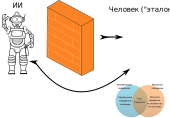
\includegraphics[width=0.9\linewidth]{pics/turing-test.pdf}
  \end{center}

  Если Человек в процессе общения с ИИ будет думать, что общается с Человеком, то ИИ обладает требуемым свойством.
\end{frame}


\begin{frame}
  \frametitle{ИИ как модель человека}
  \begin{center}
    Модулирование рассуждений \to\ моделирование <<математики>>\\
    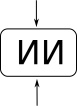
\includegraphics[width=0.2\linewidth]{pics/ai-approach.pdf}\\
    Моделирование мозга \to\ моделирование\\ самоорганизующихся систем
  \end{center}
%   \textbf{ИИ как математическая модель}
\end{frame}

\begin{frame}
  \frametitle{Свойства и классы задач ИИ}
  \small
\begin{columns}
  \begin{column}{0.4\textwidth}
    \textbf{Свойства задач}
    \begin{itemize}
    \item Не существует алгоритма решения
    \item Обработка символьной информации
    \item Автоматизация принятия решения
    \item Решение -- комбинация <<возможностей>>
    \item Обработка неполной и противоречивой информации
    \end{itemize}
    \vspace{6.5em}
    \mbox{}
  \end{column}
  \begin{column}{0.6\textwidth}
    \textbf{Классы задач}
    \begin{enumerate}
    \item Восприятие и распознавание образов
    \item Автоматическое доказательство теорем
    \item Игры
    \item Планирование действий (Problem Solving)
    \item Понимание естественного языка, перевод
    \item Логическое программирование
    \item Экспертные системы
    \item Интеллектные информационные системы
    \item Восприятие и усвоение знаний (Machine learning)
    \item Интеллектное управление [производством] \ldots
    \item Робототехника (Robotics)
    \item Системы поддержки принятия решений
    \end{enumerate}
  \end{column}
\end{columns}
\end{frame}

\begin{frame}
  \frametitle{Планирование действий (Problem Solving)}

\begin{columns}
  \begin{column}{0.4\textwidth}
    \includegraphics[width=1\linewidth]{pics/boxes.png}
  \end{column}
  \begin{column}{0.4\textwidth}
    \includegraphics[width=1\linewidth]{pics/boxes-state-space.png}
  \end{column}
\end{columns}
\vfill
\textbf{Формализованная постановка} ($SSG$, State Space Graph)
\begin{itemize}
\item Структура данных для представления \textbf{состояния}
\item Формализация \textbf{правил перехода} из состояния в состояние $G$
\item Программирование \textbf{распознавателя \emph{целевого состояния}} $R(v)$
\item Задание \textbf{исходного состояния} $I$
\end{itemize}
\vspace{1em}
\[
  SSG = <G, R(v), I>, G=<V,E>, v\in V.
\]
\end{frame}

% \begin{frame}
%   \frametitle{Игры}
% \end{frame}


\begin{frame}[fragile]
  \frametitle{Представление знаний}
\small
Естественно определить данные как некоторые сведения об отдельных объектах, а знания~-- о мире в целом.

{\bf Данные} представляют информацию о существовании объектов, представляемых значениями признаков, а {\bf знания}~-- информацию о существующих в мире закономерных связях между признаками и запрещающих некоторые другие сочетания свойств у объектов.

{\bf Данные}~-- это информация о существовании объектов с некоторым набором свойств, {\bf знания}~-- информация о несуществовании объектов с некоторым набором свойств.

Пусть $H(x)$ $\Leftrightarrow$ <<$x$~является человеком>>, а $M(x)$~-- <<$x$~-- смертен>>. \\

\noindent{}<<существует $x$, $x$ является человеком>>:
$$
    A_1=\exists x H(x),
$$
<<не существует бессмертных людей>>):
$$
    A_2=\neg\exists x \big ( H(x) \& \neg M(x) \big ),
$$
преобразуем во <<все люди смертны>>:
$$
    A_3=\forall x \big ( H(x)\to M(x)\big ).
$$
\ldots все объекты $x$, обладающие свойством $H$, будут обладать свойством $M$.

\end{frame}

\begin{frame}[fragile]
  \frametitle{Обработка информации <<в математике>>}
\small
Добавим информатики. Утверждение <<Сократ~-- человек>> представим как $H(s)$, где $s$ -- это Сократ.  Теперь из \textbf{знания} $A_3$ и \textbf{исходного данного} $H(s)$ получим новую информацию о Сократе:
$$
B = \Big (H(s) \& \overbrace{\forall x \big ( H(x)\to M(x)\big )}^{A_3} \Big ) \to M(s).
$$

Из того, что Сократ~-- человек и что все люди смертны, следует, что Сократ тоже смертен $M(s)$.  Доказательство <<от противного>>:

\begin{enumerate}
\item Требуется \textbf{опровергнуть высказывание} $\neg B = \Tr$
\item $B = \Fa \vdash$ $H(s) \& A_3 = \Tr$, $M(s) = \Fa$
\item $A_3 = \Tr \vdash H(s) = \Tr$, {\color{red}$A_3 = \Tr$} \label{pa}
\item Подставим $s$ вместо $x$ в $A_3$, получим $H(s)\to M(s)$
\item $H(s)= \Tr, M(s)= \Fa \vdash H(s)\to M(s) = \Fa$
\item $H(s)\to M(s) = \Fa\vdash$ {\color{blue} $A_3 = \Fa$} \label{pb}
\item Из п.~\ref{pa} следует {\color{red}$A_3 = \Tr$}, а из п.~\ref{pb} -- {\color{blue} $A_3 = \Fa$} \label{contr}
\item В формальной (математической) логике в п.~\ref{contr} получено \textbf{противоречие}
\item Следовательно, $\neg B \neq \Fa$, $B = \Tr$ \label{stmt}
\item Из п.~\ref{stmt} следует $M(s)=\Tr$ \square\ \ \ (\textbf{ЧТД, QED\footnote{\emph{Quod Erat Demonstrandum}, <<что и требовалось показать>>, ``which was to be demonstrated``})}
% \begin{align*}
% 2x - 5y &=  8 \\
% 3x + 9y &=  -12
% \end{align*}
\end{enumerate}
\end{frame}

\begin{frame}[fragile]
  \frametitle{Логическое программирование}

  \textbf{Сократим доказательство}

  Будем выписывать только \textbf{истинные высказывания}, т.е.
  $M(s) \Leftrightarrow M(s) = \Tr$ (<<Сократ смертен>>),\\
  $\neg M(s) \Leftrightarrow M(s) = \Fa$ (<<Сократ бессмертен>>)

$$
B = \Big (H(s) \& \overbrace{\forall x \big ( H(x)\to M(x)\big )}^{A_3} \Big ) \to M(s).
$$

\begin{columns}
  \begin{column}{0.5\textwidth}\footnotesize
    \begin{enumerate}
    \item \textbf{Опровергаем} $\neg B$
    \item $B\vdash$ $H(s) \& A_3$, $M(s)$
    \item $A_3 \vdash H(s)$, {\color{red}$A_3$} \label{pa}
    \item $A_3\{s/x\} = H(s)\to M(s)$
    \item $H(s), \neg M(s) \vdash \neg (H(s)\to M(s))$
    \item $\neg(H(s)\to M(s))\vdash$ {\color{blue} $\neg A_3$} \label{pb}
    \item Из п.~\ref{pa} следует {\color{red}$A_3$}, а из п.~\ref{pb} -- {\color{blue} $\neg A_3$} \label{contr}
    \item В п.~\ref{contr} получено \textbf{противоречие}
    \item Следовательно, $B$ \label{stmt}
    \item Из п.~\ref{stmt} $M(s)$ \square
    \end{enumerate}
    \vspace{2.7em}
    \mbox{}
  \end{column}
  \begin{column}{0.5\textwidth}
    \textbf{\footnotesize Программа (теория)}
\begin{minted}{prolog}
h(s).
m(X) :- h(X).   % h(x) -> m(x).
\end{minted}
    \textbf{\footnotesize Консультация}
\begin{minted}{text}
?- [socrates].  % Загрузка теории из файла
true.

?- m(s).        % Запрос
true.
\end{minted}
\textbf{\footnotesize Объяснение вывода}
\begin{minted}{text}
?- trace.
true.

[trace]  ?- m(s).
   Call: (10) m(s) ?     % Запрос пользователя
   Call: (11) h(s) ?     % Применение m(X):-h(X)
                         % при {s/X}
   Exit: (11) h(s) ?     % Найден факт h(s).
   Exit: (10) m(s) ?     % следовательно m(s).
true.

[trace]  ?-
\end{minted}
  \end{column}
\end{columns}
\end{frame}

\begin{frame}[fragile]
  \frametitle{Планирование действий}
  \begin{center}
    \includegraphics[width=0.7\linewidth]{pics/maze.pdf}
  \end{center}
\begin{columns}
  \begin{column}{0.5\textwidth}
  \textbf{Теория лабиринта}
\begin{minted}{prolog}

% "Данные"

e(a,b). e(b,c). e(c,f).
e(f,e). e(e,d). e(d,h).
e(f,g). e(g,i). e(i,h).

% "Знания"
% Что такое "путь".

path(A,B) :- e(A,B).
path(A,B) :- e(A,C), path(C,B).

\end{minted}

  \noindent\textbf{Запрос}

\begin{minted}{text}
?- path(a,h).
true ;
true ;
false.
\end{minted}
\end{column}
\begin{column}{0.5\textwidth}
\textbf{Конструктивное решение}
\begin{minted}{prolog}
path(A,B, [A-B]) :- e(A,B).
path(A,B, [A-C|T]) :- e(A,C), path(C,B,T).
\end{minted}
\textbf{Запрос}
\begin{minted}{text}
?- path(a,h,L).
L = [a-b, b-c, c-f, f-e, e-d, d-h] ;
L = [a-b, b-c, c-f, f-g, g-i, i-h] ;
false.
\end{minted}
\vspace{4em}
\mbox{}
\end{column}
\end{columns}
\end{frame}

\begin{frame}[fragile]
  \frametitle{Стратегии поиск в SSG}
  \begin{center}\tiny
    \def\svgwidth{0.8\linewidth}
    \def\za{A}
    \def\zb{B}
    \def\zc{C}
    \def\ya{a)}
    \def\yb{b)}
    \def\yc{c)}
    \input{pics/searchdescr.pdf_tex}
  \end{center}
\begin{columns}
  \begin{column}{0.5\textwidth}
    \textbf{Поиск в глубину}
\begin{minted}{prolog}
dfs(V,[]):- r(V).
dfs(V,[V-N|T]):- \+ r(V), after(V,N), dfs(N,T).
r(h).
after(X,Y):- e(X,Y); e(Y,X).
\end{minted}
\begin{minted}{text}
?- dfs(a, S).
S = [a-b, b-c, c-f, f-e, e-d, d-h] ;
S = [a-b, b-c, c-f, f-e, e-d, d-e, e-d, d-h] ;
S = [a-b, b-c, c-f, f-e, e-d, d-e, e-d, d-e, ...]
\end{minted}
    %\vspace{1em}
    \mbox{}
  \end{column}
  \begin{column}{0.5\textwidth}
    \textbf{Поиск в ширину}
\begin{minted}{prolog}
bfs([[X|T]|_],[X|T]):-r(X),!.   % (1)
bfs([[X|T]|Ways], S):-
    findall([Y,X|T],            % (2)
      (after(X,Y), \+ member(Y,[X|T])),
    L),
    append(Ways, L, NWays),     % (3)
    bfs(NWays, S).
\end{minted}
\begin{minted}{text}
?- bfs([[a]],S).
S = [h, d, e, f, c, b, a].
\end{minted}
  \end{column}
\end{columns}
\end{frame}

\begin{frame}[fragile]
  \frametitle{Использование дополнительной информации}
  \begin{columns}
    \begin{column}{0.5\textwidth}\footnotesize
      Зададим функцию $f\!\!:V\to R$ следующего вида:
\begin{equation*}
  % \label{eq:1}
  f(x)=g(x)+r(x)
\end{equation*}
-- стоимость кратчайшего пути (КП) через $x$,  $g(x)$~-- до $x$, $r(x)$~-- КП до целевой вершины (не известен).

Оценка $r(x)$ снизу -- $h(x)$, $h(x)\leqslant r(x)$.  Теперь
\begin{equation*}
  %\label{eq:2}
  f(x)\leqslant g(x)+h(x).
\end{equation*}
    \end{column}
    \begin{column}{0.5\textwidth}
\begin{minted}{prolog}
bf1([_-s(G,[Target|T]) |_],% (1)
    Target-_,s(G,[Target|T])):-!.
bf1([_-s(G,[X|T])|Ways], Target-GPS, S):-
    Target\=X,
    findall(F1-s(G1,[Y,X|T]),
      after([X|T],G,GPS, Y,G1,F1), L),
    append(L, Ways, NWays), keysort(NWays,SNWays),
    bf1(SNWays,Target-GPS,S).
after([S|R],SG, GPS, T,TG, F):-
    transdist(S,T,D), % \+ member(T,[S|R]),
    TG is SG + D,
    geodist(T, GPS, GDist), % (2)
    F is TG + GDist.
bf(Start, Target, Sol):-
    geocode(Target, Lon, Lat, _),
    bf1([0-s(0,[Start])],
        Target-ll(Lon,Lat), Sol). % (3)
\end{minted}
    \end{column}
  \end{columns}
  \begin{center}
    \includegraphics[width=0.7\linewidth]{pics/yuzd1.pdf}
  \end{center}
\end{frame}

\begin{frame}[fragile]
  \frametitle{Игра 15}
  \begin{columns}
    \begin{column}{0.5\textwidth}
      \includegraphics[width=1\linewidth]{pics/15-puzzle_magical.pdf}
    \end{column}
    \begin{column}{0.5\textwidth}
\textbf{Поиск решения с использованием эвристики}
\begin{minted}{text}
center% ./15-solve 100 20 1
Environment:
USE_HEURISTIC=1
Puzzle 15 solving program
State(00,00[00])
<---solution--->
0 Step ------------
 5  1  3  4
 9  2  6  8
13 10 15  0
14 12  7 11
x=2, y=3
State(00,16[16])
. . . . . .
17 Step ------------
 1  2  3  4
 5  6  7  8
 9 10 11 12
13 14 15  0
x=3, y=3
State(17,00[17])
Tested 111 states.
\end{minted}
\textbf{Без эвристики}
\begin{minted}{text}
. . . . . .
17 Step ------------
 1  2  3  4
 5  6  7  8
 9 10 11 12
13 14 15  0
x=3, y=3
State(17,00[17])
Tested 921299 states.
\end{minted}
    \end{column}
  \end{columns}
\end{frame}

\begin{frame}
  \frametitle{Понимания естественного языка: актуальность}
  \footnotesize
  Понимание естественного языка (ЕЯ), перевод из одного ЕЯ на другой -- \textbf{Направление ИИ}. Решаются следующие задачи:
  \begin{enumerate}
  \item Анализ текстов, помещение изъятой информации в базу данных:
    \begin{itemize}
    \item изготовление шаблонов документов, отчетов;
    \item синтез структур данных для ИС;
    \item заполнение баз данных ИС и т.п.;
    \end{itemize}
  \item Ведение диалога с пользователем:
    \begin{itemize}
    \item идентификация моделей и планирование действий (интеллектные пользовательские интерфейсы);
    \item приобретение знаний (оболочки экспертных систем);
    \end{itemize}
  \item Управление приложением:
    \begin{itemize}
    \item запросы на естественном языке к базам данных;
    \item внесение изменений в данные;
    \item командное управление (<<Проветрить квартиру>>).
    \end{itemize}
  \end{enumerate}
  % Цель лекции -- рассмотреть методику использования ЕЯ в качестве языка запросов к базе данных.
\end{frame}

\begin{frame}
  \frametitle{Графический пользовательский интерфейс}
  Специализирован на \textbf{операциях над отдельными частями} информационного объекта.
  \begin{center}
    \includegraphics[width=0.4\linewidth]{pics/shot-context-menu.png}\qquad
    \includegraphics[width=0.4\linewidth]{pics/shot-replace.png}
  \end{center}
  В операциях аргументы вводится в диалоговом окне (для операций с аргументами).

  Более <<умные>> редакторы не используют контекстные операции (EMACS, VI, Visual Studio Code, Sublime, AutoCAD).
\begin{quote}
  \texttt{Alt-X replace-string}, Набирается как <<Alt-X repl str>>
\end{quote}
\begin{center}
    \includegraphics[width=0.9\linewidth]{pics/shot-replace-string-emacs.png}\qquad
  \end{center}
\end{frame}

\begin{frame}
  \frametitle{Язык как математическая модель}
  \begin{block}{Семиотика (наука о знаках) делится на три раздела (Моррис)}
  \begin{itemize}
  \item \textbf{Семантика} — отношение знака к объекту: \\ Что значит \emph{знак}?
  \item \textbf{Синтаксис} — отношение знаков между собой --\\ как создаются \emph{новые смыслы} (термины, суждения) комбинированием \emph{знаков}.
  \item \textbf{Прагматика} — отношение знака к субъекту:\\ Что \emph{обозначает предложение}, что надо дальше делать? На какой конкретно вопрос и как надо отвечать?
  \end{itemize}
\end{block}
\end{frame}

\begin{frame}
  \frametitle{Язык программирования}
\textbf{Синтаксис} на уровне грамматики определяет корректные последовательности символов (операторы, структуры). Но синтаксическая правильность не гарантирует даже осмысленности программы. % Таким образом, синтаксис определяет лишь одну сторону языка.

\textbf{Семантика} — это соответствие между синтаксически правильными программами и [вариантами] действий абстрактного исполнителя, то есть это смысл синтаксических конструкций.

\textbf{Прагматика} задает конкретизацию абстрактного вычислителя (конкретный процессор и др. ресурсы) для  вычислительной системы. Стандарт языка программирования задаёт поведение вычислителя не полностью, конкретный транслятор языка переводит программу в конкретной машинный код на конкретную программно-аппаратную платформу.

Реализованный язык является прагматическим опосредованием абстрактной модели вычислений и ее реализацией на конкретном компьютере.
\vfill
\textbf{Цель программиста} — получить нужный ему эффект в результате исполнения программы на конкретном оборудовании: трансляция и исполнение осуществляется на конкретных вычислителях.

\end{frame}

\begin{frame}
  \frametitle{Синтаксический разбор предложения}
  \begin{center}
    \includegraphics[width=1\linewidth]{pics/morphosent.pdf}
  \end{center}
\end{frame}

\begin{frame}
  \frametitle{Грамматика}
   \begin{columns}
     \begin{column}{0.6\textwidth}
       \begin{block}{}
       \[
         G=\langle T,N,\Sigma,R\rangle
       \]
     \end{block}
       $T$ -- множество терминальных символов (слова, буквы, \texttt{IF}, \texttt{ELSE}),\\
       $N$ -- множество нетерминальных символов (обозначения, $\Alpha, \Beta$, <noun>, <verb>), $T\cap N=\emptyset,$\\
       $\Sigma$ -- стартовый символ (<программа>, <предложение>), $\Sigma\in N,$\\
       $R$ -- множество правил грамматики $\Alpha\to\Beta$, \\$R\subset((T\cup N)^* N(T \cup N)^*)\times(T\cup N)^*$.\\[0.5em]
       Язык $L(G)=\{\Omega\in T^* | \Sigma\to^*\Omega\}$.
     \end{column}
     \begin{column}{0.4\textwidth}
       \begin{block}{Вывод $\Sigma\to^*\Omega$}
         \[\Sigma\to\Sigma\Alpha\quad \Sigma\to\Alpha\]
         \[\Alpha\to b\Sigma e\quad \Alpha\to be \]
         Пример: \(a=`(',\quad b=`)'\).
         \begin{raggedleft}
           \[
             \begin{array}{ll}
               \Sigma & \Sigma\\
               \Alpha & \Alpha\\
               b\Sigma e & ( \Sigma )\\
               b\Sigma\Alpha e & ( \Sigma\Alpha )\\
               b\Alpha\Alpha e & ( \Alpha\Alpha )\\
               bbe\Alpha e & (() \Alpha )\\
               bbebee & (()())
             \end{array} \]
         \end{raggedleft}
     \end{block}
     \end{column}
   \end{columns}
\end{frame}

\begin{frame}
  \frametitle{Типы грамматик}
  По иерархии Ноама Хомского, грамматики делятся на \textbf{четыре} типа, каждый последующий является более ограниченным подмножеством предыдущего (но и легче поддающимся анализу):
  \begin{itemize}
    \item Тип 0. Неограниченные грамматики — возможны любые правила;
    \item Тип 1. Контекстно-зависимые грамматики — левая часть может содержать один нетерминал, окруженный «контекстом»; сам нетерминал заменяется непустой последовательностью символов в правой части;
    \item Тип 2. Контекстно-свободные грамматики — левая часть состоит из одного нетерминала;
    \item Тип 3. Регулярные грамматики — более простые, распознаются конечными автоматами.
  \end{itemize}
\end{frame}

\begin{frame}[fragile]
  \frametitle{Грамматика языка программирования С}
  {\ltprgsize
 \begin{verbatim}
<translation-unit> ::= {<external-declaration>}*

<external-declaration> ::= <function-definition>
                   | <declaration>

<function-definition> ::= {<declaration-specifier>}* <declarator> {<declaration>}* <compound-statement>
                   | union

<struct-declaration> ::= {<specifier-qualifier>}* <struct-declarator-list>
. . . . . .
<specifier-qualifier> ::= <type-specifier>
                   | <type-qualifier>

<struct-declarator-list> ::= <struct-declarator>
                   | <struct-declarator-list> , <struct-declarator>

<struct-declarator> ::= <declarator>
                   | <declarator> : <constant-expression>
                   | : <constant-expression>
. . . . . .
<selection-statement> ::= if ( <expression> ) <statement>
                   | if ( <expression> ) <statement> else <statement>
                   | switch ( <expression> ) <statement>

<iteration-statement> ::= while ( <expression> ) <statement>
                   | do <statement> while ( <expression> ) ;
                   | for ( {<expression>}? ; {<expression>}? ; {<expression>}? ) <statement>

<jump-statement> ::= goto <identifier> ;
                   | continue ;
                   | break ;
                   | return {<expression>}? ;
\end{verbatim}}
\end{frame}

\begin{frame}[fragile]
  \frametitle{Пример трансляции}
   \begin{columns}
     \begin{column}{0.5\textwidth}
 \begin{minted}{c}
#include <stdio.h>

typedef unsigned long int ulint;

ulint fact (ulint n) {
    if (n==0) return 1;
    if (n==1) return 1;
    return n*fact(n-1);
}

int main() {
    ulint n = 10;
    printf("Factorial of %lu = %lu.\n",
        n, fact(n));
    return 0;
}
 \end{minted}
     \end{column}
      \begin{column}{0.5\textwidth}
\begin{minted}{asm}
	.file   "fact.c"
	.text
	.globl  fact
	.type   fact, @function
fact:
.LFB11:
	movl    $1, %eax
	cmpq    $1, %rdi
	jbe     .L4
.L3:
	imulq   %rdi, %rax
	subq    $1, %rdi
	cmpq    $1, %rdi
	jne    .L3
.L4:
	ret
.LFE11:
	.section    .rodata.str1.1,"aMS",@progbits,1
.LC0:
	.string     "Factorial of %lu = %lu.\n"
	.section    .text.startup,"ax",@progbits
	.globl  main
	.type   main, @function
main:
.LFB12:
	;; . . . . . . . . . . .
	ret
	.cfi_endproc
.LFE12:
	.size   main, .-main
	.ident  "GCC: (GNU) 8.2.1 20181127"
	.section    .note.GNU-stack,"",@progbits
\end{minted}
      \end{column}
    \end{columns}
 \end{frame}

\begin{frame}[fragile]
  \frametitle{Синтаксический разбор предложения}
  Корова трясет хвостом.\\
  A cow shakes the tail.

  \verb|% [a, cow, shakes, the, tail]|

  \textbf{Грамматика:}
  \begin{itemize}
  \item Множество \textbf{терминальных} символов -- \{a,b,c,\ldots,z\}.  На самом деле, $\Sigma=\{a,cow,shakes,walks,\ldots\}$.
  \item Множество \textbf{нетерминальных} символов -- \texttt{<sentence>, <noun>, <verb>, \ldots}
  \item \textnormal{Стартовый} символ -- \texttt{<sentence>}.
  \item \textbf{Правила} упрощенного английского языка:
    \begin{align}
      \label{eq:eng-gramm}
      \langle{}sentence\rangle{} & \to  \langle{}noun group\rangle{} \langle{}verb group\rangle{} \\
      \langle{}noun group\rangle{} & \to  \langle{}determinant\rangle{} \langle{}noun\rangle{} \\
      \langle{}verb group\rangle{} & \to  \langle{}verb\rangle{} \langle{}noun group\rangle{} \\
      \langle{}noun\rangle{} & \to cow\ |\ tail\ |\ \ldots \\
      \langle{}verb\rangle{} & \to walks\ |\ shakes\ |\ \ldots \\
      \langle{}determinant\rangle{} & \to a\ |\ the\ |\ \varepsilon\ |\ my\ |\ \ldots
    \end{align}
  \end{itemize}
\end{frame}


\begin{frame}
  \frametitle{Linked grammar (грамматики связей)}
  \begin{columns}
    \begin{column}{0.4\textwidth}
      \includegraphics[width=0.9\linewidth]{pics/l-g-parts.png}
      \includegraphics[width=0.9\linewidth]{pics/l-g-table.png}
    \end{column}
    \begin{column}{0.6\textwidth}
      Последовательность слов находится в linked grammar, если существует способ нарисовать связи между словами, такие что\\[1em]
%      Sequence of words is in the language of link grammar if there is a way to draw links between words in such a way that

      Связи не пересекаются (\textbf{планарный граф});\\[0.5em]
      Все слова последовательности соединены связями (\textbf{связность});\\[0.5em]
      Все связи удовлетворяют ограничениям (\textbf{непротиворечивость})\\[0.5em]
      Два слова соединены одной и только одной связью (\textbf{исключительность}).\\[0.5em]
    \end{column}
  \end{columns}
\end{frame}

\begin{frame}
  \frametitle{Примеры разбора Linked grammar}
  \centering
  “The cat chased a snake”\\
  \includegraphics[width=0.6\linewidth]{pics/l-g-good-ex.png}\\[1em]
  “The Mary chased cat”\\
  \includegraphics[width=0.6\linewidth]{pics/l-g-bad-ex.png}
\end{frame}

\begin{frame}
  \frametitle{Примеры разбора Linked grammar}
  \centering
  “A dog arrived with a bone”\\
  “A dog with a bone arrived”\\
  \includegraphics[width=0.6\linewidth]{pics/l-g-multi-ex.png}\\[1em]
\end{frame}

\begin{frame}
  \frametitle{Примеры разбора Linked grammar}
  \centering
  \includegraphics[width=0.8\linewidth]{pics/l-g-prog-ex.png}\\[1em]
\end{frame}

\begin{frame}[fragile,fragile]
  \frametitle{Информационная система GeoBase. База данных}
  GeoBase -- программа, позволяющая делать запросы на ЕЯ к базе данных по географии США, Borland, 1988.
\begin{minted}{prolog}
state('alabama','al','montgomery',3894e3,51.7e3,22,'birmingham','mobile','montgomery','huntsville').
state('alaska','ak','juneau',401.8e3,591e3,49,'anchorage','fairbanks','juneau','sitka').

city('alabama','al','birmingham',284413).
city('alabama','al','mobile',200452).

border('florida','fl',['georgia','alabama']).

highlow('alabama','al','cheaha mountain',734,'gulf of mexico',0).

mountain('alaska','ak','mckinley',6194).
mountain('alaska','ak','st. elias',5489).

road('66',['district of columbia','virginia']).

lake('huron',59570,['michigan']).
\end{minted}
  {\ttfamily\ltprgsize
\begin{verbatim}


  The database contains the following information:

Information about states:
  Area of the state in square kilometers
  Population of the state in citizens
  Capital of the state
  Which states border a given state
  Rivers in the state
  Cities in the state
  Highest and lowest point in the state in meters

Information about rivers:
  Length of river in kilometers

Information about cities:
  Population of the city in citizens
\end{verbatim}}
\end{frame}

\begin{frame}[fragile]
   \frametitle{Примеры запросов}
{\ttfamily\footnotesize
\begin{verbatim}
Some sample queries:

   - states

   - give me the cities in california.

   - what is the biggest city in california ?

   - what is the longest river in the usa?

   - which rivers are longer than 1 thousand kilometers?

   - what is the name of the state with the lowest point?

   - which states border alabama?

   - which rivers do not run through texas?

   - which rivers run through states that border the state
     with the capital austin?
\end{verbatim}}
\end{frame}

\begin{frame}[fragile]
  \frametitle{Схемы (спецификации) интерпретации}
  \begin{columns}
    \begin{column}{0.4\textwidth}
\begin{minted}{prolog}
schema('abbreviation','of','state').
schema('state','with','abbreviation').
schema('capital','of','state').
schema('state','with','capital').
schema('population','of','state').

schema('area','of','state').
schema('city','in','state').

schema('length','of','river').
schema('state','with','river').
schema('river','in','state').

schema('capital','with','population').
schema('point','in','state').

schema('height','of','point').
schema('mountain','in','state').

schema('height','of','mountain').
schema('lake','in','state').

schema('name','of','river').
schema('name','of','capital').

schema('road','in','continent').
\end{minted}
    \end{column}
    \begin{column}{0.6\textwidth}
      \includegraphics[width=1\linewidth]{pics/sem-net-1.pdf}
    \end{column}
  \end{columns}
\end{frame}

\begin{frame}[fragile]
  \frametitle{Программа}
  Основной цикл программы
\begin{minted}{prolog}
geobase(STR, X, E):-
        STR \= "",
        atom_string(ATOM,STR),
        tokenize_atom(ATOM,LIST),     /* Returns a list of words(symbols)           */
        filter(LIST,LIST1),           /* Removes punctuation and words to be ignored*/
        pars(LIST1,E,Q),              /* Parses queries                            */
        findall(A,eval_interp(Q,A),L),
        unik(L,L1),
        % unit(E,U),
        member(X,L1).
\end{minted}
  Синтаксический анализатор (часть)
\begin{minted}{prolog}
  pars(LIST,E,Q):-s_attr(LIST,OL,E,Q),check(OL),!.
  pars(LIST,_,_):-error(LIST),fail.
% . . . . . .
  /* How big is the biggest city -- BIG QUERY */
  s_attr([BIG|S1],S2,E1,q_eaq(E1,A,E2,Q)):-
		size(_,BIG),s_minmax(S1,S2,E2,Q),
		size(E2,BIG),entitysize(E2,E1),
		schema(E1,A,E2),!.

  s_attr(S1,S2,E,Q):-s_minmax(S1,S2,E,Q).
% . . . . . .

/* ... the shortest river in texas -- MIN QUERY */
  s_assoc1([MIN|S1],S2,E1,A,q_eaq(E1,A,E2,q_min(E2,Q))):-minn(MIN),!,
		s_nest(S1,S2,E2,Q),schema(E1,A,E2).

/* ... the longest river in texas -- MAX QUERY */
  s_assoc1([MAX|S1],S2,E1,A,q_eaq(E1,A,E2,q_max(E2,Q))):-maxx(MAX),!,
		s_nest(S1,S2,E2,Q),schema(E1,A,E2).
\end{minted}
\end{frame}

\begin{frame}[fragile]
  \frametitle{Корпус, источник данных}
  \texttt{population of Washington}\\
  Население штата или города?\\
  \textbf{?-} \texttt{schema('population','of','city').}\\
  \textbf{?-} \texttt{schema('population','of','state').}\\
  Корпус реализован при помощи реструктуризации базы данных.
\begin{minted}{prolog}
  % . . . . . . . . .
  /* Relationships about states */
  db(abbreviation,of,state,ABBREVIATION,STATE):-  state(STATE,ABBREVIATION,_,_,_,_,_,_,_,_).
  db(state,with,abbreviation,STATE,ABBREVIATION):-state(STATE,ABBREVIATION,_,_,_,_,_,_,_,_).
  db(area,of,state,AREA,STATE):-        state(STATE,_,_,_,AREA1,_,_,_,_,_),str_real(AREA,AREA1).
  db(capital,of,state,CAPITAL,STATE):-  state(STATE,_,CAPITAL,_,_,_,_,_,_,_).
  db(state,with,capital,STATE,CAPITAL):-state(STATE,_,CAPITAL,_,_,_,_,_,_,_).
  db(population,of,state,POPULATION,STATE):-state(STATE,_,_,POPUL,_,_,_,_,_,_),str_real(POPULATION,POPUL).
  db(state,border,state,STATE1,STATE2):-border(STATE2,_,LIST),member(STATE1,LIST).

  /* Relationships about rivers */
  db(length,of,river,LENGTH,RIVER):-    river(RIVER,LENGTH1,_),str_real(LENGTH,LENGTH1).
  db(state,with,river,STATE,RIVER):-    river(RIVER,_,LIST),member(STATE,LIST).
  db(river,in,state,RIVER,STATE):-      river(RIVER,_,LIST),member(STATE,LIST).

  /* Relationships about points */
  db(point,in,state,POINT,STATE):-      highlow(STATE,_,POINT,_,_,_).
  db(point,in,state,POINT,STATE):-      highlow(STATE,_,_,_,POINT,_).
  db(state,with,point,STATE,POINT):-    highlow(STATE,_,POINT,_,_,_).
  db(state,with,point,STATE,POINT):-    highlow(STATE,_,_,_,POINT,_).
  db(height,of,point,HEIGHT,POINT):-    highlow(_,_,_,_,POINT,H),str_real(HEIGHT,H),!.
  db(height,of,point,HEIGHT,POINT):-    highlow(_,_,POINT,H,_,_),str_real(HEIGHT,H),!.
  % . . . . . . . . .
\end{minted}
\end{frame}

\begin{frame}[fragile]
  \frametitle{Программа}
  Интерпретация запроса \texttt{\ldots findall(A,eval\_interp(Q,A),L), \ldots}
\begin{minted}{prolog}
  eval_interp(Q,IAns):-
		eval(Q,A),
		e_i(A,IAns).

  eval(q_min(ENT,TREE),ANS):-
		findall(X,eval(TREE,X),L),
		entitysize(ENT,ATTR),
		sel_min(ENT,ATTR,99e99,'',ANS,L).

  eval(q_max(ENT,TREE),ANS):-
		findall(X,eval(TREE,X),L),
		entitysize(ENT,ATTR),
		sel_max(ENT,ATTR,-1,'',ANS,L).

  eval(q_sel(E,gt,ATTR,VAL),ANS):-
		schema(ATTR,ASSOC,E),
		db(ATTR,ASSOC,E,SVAL2,ANS),
		str_real(SVAL2,VAL2),
		VAL2>VAL.
% . . . . . . .
  eval(q_eaq(E1,A,E2,TREE),ANS):-
		eval(TREE,VAL),db(E1,A,E2,ANS,VAL).

  eval(q_eaec(E1,A,E2,C),ANS):-db(E1,A,E2,ANS,C).

  eval(q_e(E),ANS):-	ent(E,ANS). % EVAL "ATOM"

  eval(q_or(TREE,_),ANS):- eval(TREE,ANS).

  eval(q_or(_,TREE),ANS):- eval(TREE,ANS).

  eval(q_and(T1,T2),ANS):- eval(T1,ANS1),eval(T2,ANS),ANS=ANS1.
\end{minted}
\end{frame}

\begin{frame}[fragile]
  \frametitle{Пример запуска программы Geobase}
  \footnotesize
\begin{minted}{text}
Welcome to SWI-Prolog (threaded, 64 bits, version 9.0.4)
SWI-Prolog comes with ABSOLUTELY NO WARRANTY. This is free software.
Please run ?- license. for legal details.

For online help and background, visit https://www.swi-prolog.org
For built-in help, use ?- help(Topic). or ?- apropos(Word).

?- [geobase].
true.

?- loaddba.
Loading database file - please wait
true.

?- geobase:geobase("states").
alabama alaska arizona arkansas california
colorado connecticut delaware florida georgia
hawaii idaho illinois indiana iowa
kansas kentucky louisiana maine maryland
massachusetts michigan minnesota mississippi missouri
montana nebraska nevada new hampshire new jersey
new mexico new york north carolina north dakota
ohio oklahoma oregon pennsylvania rhode island
south carolina south dakota tennessee texas
utah vermont virginia washington west virginia
wisconsin wyoming

50 Solutions
true.

?- geobase:geobase("which rivers run through states that border the state with the capital austin?").
neosho washita arkansas st. francis white
mississippi ouachita pearl red canadian
cimarron rio grande san juan gila pecos

15 Solutions
true.
\end{minted}
\end{frame}

\begin{frame}
  \frametitle{Chat GPT}
  ChatGPT (Generative Pretrained Transformer, Порождающий [пред]треннированный Трансформатор) -- чат-бот OpenAI, запущенный в ноябре 2022.

  Настроен при помощи обучения <<с учителем>> и <<с подкреплением>>.

  Предназначен для реагирования на входные данные, представленные на естественном языке.

\end{frame}

\begin{frame}
  \frametitle{QR-код презентации}
  \centering
%  \includegraphics[width=0.7\linewidth]{pics/qrcode.eps}
\end{frame}

\end{document}

% talk-iccs-de-lect-2023-07.tex

%%% Local Variables:
%%% mode: latex
%%% TeX-master: t
%%% End:
